\lesson{1}{Jul 21 2022 Thu (17:36:02)}{Introduction to Anatomy and Physiology}
\label{les_1:introduction_to_anatomay_and_physiology}

\begin{definition}[Anatomy]
	\label{def:anatomy}

	The study of the \textbf{structure} and \textbf{relationships} between
	\textbf{body parts}.
\end{definition}

\begin{definition}[Physiology]
	\label{def:physiology}

	The science \textbf{of how those parts come together to function}, and keep
	that body alive.
\end{definition}

Together, these two create the \textbf{Science of Us}.

\subsection*{History of Anatomy}
\label{sub_sec:history_of_anatomy}

The history of anatomy is a very long and somewhat of a secretive road. In many
societies, it was considered a taboo of performing human dissections. The $2$nd
century Greek physician Galen extracted what he could about the human form by
performing dissections on pigs. Leonardo Da Vinci poked around the human
bodies, documenting them all in his beautifully sketched drawings, until the
pope made him stop. Here are some of his drawings.

\begin{figure}[H]
	\centering
	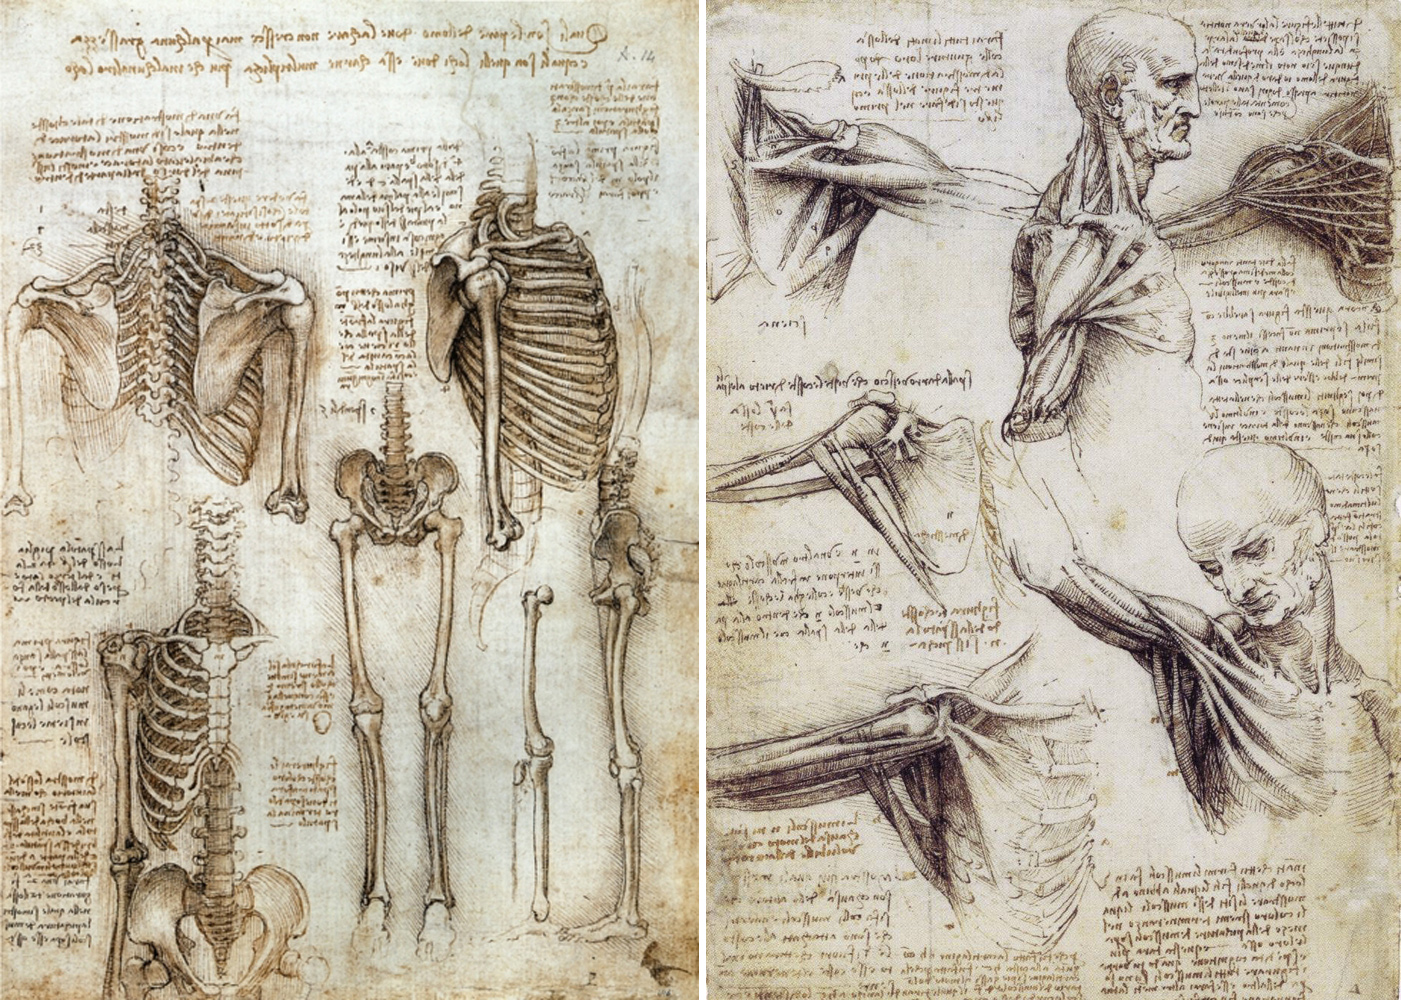
\includegraphics[width=1\textwidth]{img/da-vinci-human-drawings}
	\caption{Da-Vinci Human Sketches and Diagrams}
	\label{fig:da_vinci_human_sketches_and_diagrams}
\end{figure}

Finally, in the $17$th and $18$th centuries, certified anatomists were allowed
to perform tightly regulated human dissections. They were extremely popular. So
popular that you needed an admissions fee to view the dissection, and the likes
of Michelangelo and Rembrandt used to watch.

Eventually, the craze for human anatomy become such a craze that in Europe,
grave robbers started becoming an actual job, until $1832$, when Britain passed
the \textbf{Anatomy Act}, which provided students with plenty of corpses, in
the form of executed murderers.

Still though, today students of anatomy and physiology use educational cadavers
to learn, in person and hands-on, what's inside a human body by dissecting
them.

\begin{definition}[Cadaver]
	\label{def:cadaver}

	A \textbf{cadaver} is a volunteer who donates his/her body after their death
	to science.
\end{definition}

% subsection history_of_anatomy (end)

\subsection*{How parts functions}
\label{sub_sec:how_parts_functions}

The function of a cell or an organ or a whole organism always reflects its
form. Blood flows in one direction through your heart because its valves
prevent it from flowing the other way. In the same way, your bones are strong
and hard, which allows them to protect and support all your soft parts.

\begin{definition}[Complementarity of Structure and Function]
	\label{def:complementarity_of_structure_and_function}

	The \textbf{complementarity of structure and function} is an idea that a what
	structure can do depends on its form.
\end{definition}

This holds true for all levels of your body's organization. From cell to
tissue.

% subsection how_parts_functions (end)

\subsection*{Hierarchy of Organization}
\label{sub_sec:hierarchy_of_organization}

It all begins with the smallest of the small. \textbf{Atoms}. The next level up
from chemistry of atoms and molecules include the smallest unit of living
things -- cells. All cells have some basic functions in common, but they also
vary widely in size and shape, depending on their purpose.

\begin{example}
	\label{exm:cells}

	The \textbf{red blood cell} measures about $5$ micrometers across, which,
	when compared to the \textbf{single motor neuron} that runs from the end of
	your big toe to the bottom of your spine, which measures about a meter.
\end{example}

Typically, cells group with other cells to form the next level of organization;
\textbf{tissues}. When two or more tissues combine, they form \textbf{organs}
that performs specific functions that keep your body running. Organs work
together and combine to get things done, forming \textbf{organ systems}. And
finally, all those previous levels combine to make the final organization
level; \textbf{the body}.

\begin{definition}[Homeostasis]
	\label{def:homeostasis}

	This allows your body to maintain \textbf{stable, internal conditions} not
	matter what \textbf{changes} are occurring \textbf{outside the body}.
\end{definition}

Everyone's ultimate cause of death is the extreme and irreversible loss of
homeostasis. Organ failure, suffocation, starvation, dehydration; they all lead
to the same end, by throwing off the internal balances that allow your body to
keep processing energy.

% subsection hierarchy_of_organization (end)

\subsection*{Directional Terms}
\label{sub_sec:directional_terms}

With so many connected parts needed to make your life possible, there's a need
for a hyper-precise language to identify the parts of your body and communicate
what happening to them.

\begin{definition}[Verbal Map]
	\label{def:verbal_map}

	A \textbf{verbal map} is a detailed description of what's.
\end{definition}

When you go to get a surgery, the doctor tells the surgeon a \textbf{verbal
	map}.

\begin{definition}[Directional Terms]
	\label{def:directional_terms}

	The \textbf{directional terms} is a standardized set of directional terms
	that describe where one body part is in relation to another.
\end{definition}

\begin{definition}[Anatomical Position]
	\label{def:anatomical_position}

	The \textbf{anatomical position} is when the body is erect and facing
	forward, with arms at the sides and palms forward.
\end{definition}

\begin{figure}[H]
	\centering
	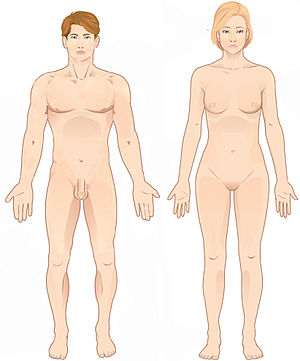
\includegraphics[width=0.5\textwidth]{img/classic-anatomical-position}
	\caption{The Classic Anatomical Position}
	\label{fig:the_classic_anatomical_position}
\end{figure}

\subsubsection*{Directional Terms}
\label{sub_sub_sec:directional_terms}

\begin{table}[H]
	\centering

	\begin{tabular}{ll}
		\textbf{Anterior}    & At or near the front of the body (front view)              \\
		\textbf{Posterior}   & At or near the back of the body (back view)                \\
		\textbf{Midline}     & An imaginary vertical line that divides the body equally   \\
		\textbf{Lateral}     & Farther from midline (side view)                           \\
		\textbf{Medial}      & Nearer to midline (side view)                              \\
		\textbf{Superior}    & Toward the head/upper part of a structure (looking down)   \\
		\textbf{Inferior}    & Away from the head/lower part of a structure (bottom view) \\
		\textbf{Superficial} & Close to the surface of the body                           \\
		\textbf{Deep}        & Away from the surface of the body                          \\
		\textbf{Proximal}    & Nearer to the origination of a structure                   \\
		\textbf{Distal}      & Farther from the origination of structure
	\end{tabular}

	\caption{All Directional Terms}
	\label{tab:all_directional_terms}
\end{table}

% subsubsection directional_terms (end)

% subsection directional_terms (end)

\newpage
